\chapter{Технологический раздел}

В данном разделе приведены средства реализации, структура программного обеспечения, листинги кода и интерфейс ПО.

\section{Средства реализации ПО}

\subsection{Выбор языка программирования}

Для реализации ПО был выбран язык программирования python [4]. Данный выбор обусловлен следующими причинами:
\begin{itemize}
	\item имеющийся опыт разработки на данном языке;
	\item python поддерживает объектно-ориентированный подход;
	\item обширный функционал языка, а также огромное количество библиотек и фреймворков, которые отлично подходят для быстрой разработки web-приложений;
	\item python имеет одно из самых больших и активных сообществ разработчиков, по нему есть большое количество литературы и информации.
\end{itemize}

\subsection{Выбор СУБД}

В роли СУБД было решено использовать PostgreSQL [5].

PostgreSQL [5] --- СУБД с открытым исходным кодом, основой которого был код, написанный в Беркли. Она поддерживает большую часть стандарта SQL и предлагает множество современных функций:

\begin{itemize}
 \item сложные запросы;
 \item поддержка многопоточности и параллелизма;
 \item внешние ключи;
 \item триггеры;
 \item изменяемые представления;
 \item транзакционная целостность;
 \item многоверсионность.
 \item поддержка восстановления после сбоев;
 \item возможность масштабируемости и репликации для дальнейшего роста интернет-магазина;
 \item является системой с открытым исходным кодом, что означает наличие большого сообщества разработчиков и пользователей, активно поддерживающих и обновляющих его.
\end{itemize}

Данный выбор обусловлен описанным выше функционалом, удовлетворяющим всем требованиям данного проекта, опытом разработки ПО с использованием данной СУБД и ее совместимостью с python.

\subsection{Выбор платформы для реализации ПО}

Для реализации ПО был выбран веб-фреймворк Django [6].
Django --- высокоуровневый веб-фреймворк, способствующий быстрой разработке и чистому, прагматичному дизайну.

Выбор данного фреймворка обусловлен такими его достоинствами, как:

\begin{itemize}
	\item автоматическая генерация административного интерфейса: Django автоматически создает административный интерфейс для управления данными в базе данных. Это упрощает администрирование и позволяет быстро создать функциональную панель управления;
	\item ORM: Django предоставляет ORM, который позволяет работать с базой данных через объектно-ориентированный интерфейс. Это позволяет разрабатывать приложения, не требуя написания SQL-запросов вручную, что сокращает время разработки и упрощает обслуживание кода;
	\item Встроенная аутентификация и авторизация: Django предоставляет функциональность для аутентификации пользователей и контроля доступа к различным частям приложения. Это помогает сделать проект безопасным и защищенным;
	\item Интеграция с другими технологиями: Django хорошо интегрируется с другими популярными технологиями и фреймворками, такими как Bootstrap, jQuery, REST framework и другими. Это позволяет использовать широкий спектр инструментов при разработке проекта;
	\item Широкое сообщество: Django имеет большое и активное сообщество разработчиков. Существует множество документации, учебных пособий, видеоуроков и форумов, посвященных Django.
	\item Встроенная защита от внешних угроз: механизмы предотвращения SQL-инъекций и подделки межсайтовых запросов;
\end{itemize}

\subsection{Выбор инструмента для работы с БД}

В качестве инструмента для работы с БД был выбран Django-ORM, так как он ключен в базовый функционал фреймворка Django и обладает следующими достоинствами:

\begin{itemize}
	\item позволяет определить модели, которые представляют таблицы в базе данных. Каждый атрибут модели соответствует полю в таблице, а методы предоставляют функциональность для работы с данными;
	\item позволяет автоматически создать схему базы данных на основе определенных моделей. Он обнаруживает изменения в моделях и создает или обновляет таблицы в соответствии с этими изменениями;
	\item предоставляет API для выполнения различных типов запросов к базе данных. Он поддерживает широкий спектр операций, таких как фильтрация, сортировка, агрегация и связи между моделями;
	\item использует концепцию ленивой загрузки данных, что означает, что запросы к базе данных выполняются только при необходимости. Это повышает производительность и уменьшает нагрузку на базу данных;
	\item поддерживает транзакции, что обеспечивает целостность данных при выполнении нескольких запросов. Он также предоставляет инструменты для создания и применения миграций, что позволяет изменять структуру базы данных без необходимости вручную редактировать схему.
\end{itemize}

Так как некоторые запросы к БД требуют вызовы функций базы, а Django-ORM, к сожалению, не поддерживает данный функционал, они были реализованы на чистом SQL. SQL-запросы отправлялись с помощью встроенного функционала Django, реализованного с использованием библиотеки \textbf{psycopg2}

\subsection{Выбор средств отображения страниц браузера}

Для отображения web-страниц в браузере был выбран HTML, CSS и JS фреймворк Bootstrap [7].

К плюсам Bootstrap можно отнести:
\begin{itemize}
	\item кросс-браузерность;
	\item единство стилей элементов;
	\item ускорение верстки сайтов в сравнении с чистым CSS и JS.
\end{itemize}

В качестве среды разработки была выбрана среда Visual Studio Code.

\section{Структура программного обеспечения}
Структура проекта задается используемым фреймворком 

Основные модули приложения:
\begin{itemize}
	\item \verb;views.py; --- содержит функции для обработки запросов к приложению и отображению нужных веб-страниц;
	\item \verb;models.py; --- содержит классы, соответствующие таблицам базы данных для работы Django ORM и менеджеры, включающие функции запросов к данным таблицам;
	\item \verb;forms.py; --- содержит классы обработки и валидации форм;
	\item \verb;urls.py; --- содержит URL-адреса страниц приложения и соответствующие им обработчики;
	\item \verb;cart.py; --- содержит класс корзины товаров пользователя;
	\item \verb;admin.py; --- содержит параметры страницы администрирования приложения.
\end{itemize}

\section{Листинги кода}

\subsection{Создание базы данных}

В приложении была создана база данных, соответствующая описанию, приведенному в аналитическом и конструкторских отделах. Создание базы данных было реализованы с помощью Django ORM и механизмом миграций Django [6].

Код описания классов таблиц представлен в приложении A.

Также на поля таблиц были наложены ограничения, представленные в приложении B.

\subsection{Функции}

Для работы приложения было создано две функции:

\begin{itemize}
	\item \verb;popular_products(); --- функция получения id товаров, отсортированных по популярности. Под популярностью подразумевается количество вхождений в заказы пользователей.
	\item \verb;total_price(integer); --- функция расчета полной стоимости заказа. На вход функция получает id заказа, на выход возвращает полную стоимость с учетом количества каждого товара в заказе.
\end{itemize}

На листинге \ref{popular_products} представлена функция \verb;popular_products();.

\captionsetup{singlelinecheck = false, justification=raggedright}
\begin{lstlisting}[label=popular_products,caption=Функция получения популярных товаров]
CREATE OR REPLACE FUNCTION popular_products()
RETURNS TABLE (
    product int
) AS $$
BEGIN
    DROP TABLE IF EXISTS popular_products;

    CREATE TEMP TABLE popular_products(
        product int
    );

    INSERT INTO popular_products (product)
    WITH tmp AS (
	SELECT product_id, COUNT(app_orders_products.id) AS count_products
	FROM app_orders_products
	GROUP BY product_id
	ORDER BY count_products DESC)
    SELECT product_id FROM tmp;

    RETURN QUERY SELECT * FROM popular_products;
END;
$$ language PLPGSQL;
\end{lstlisting}

На листинге \ref{total_price} представлена функция \verb;total_price(integer);.

\newpage

\captionsetup{singlelinecheck = false, justification=raggedright}
\begin{lstlisting}[label=total_price,caption=Функция получения общей суммы заказа по его id]
CREATE OR REPLACE FUNCTION total_price(integer)
RETURNS INT AS $$
BEGIN
    RETURN (WITH TMP(product_id, cost, cnt, total) AS 
        (SELECT product_id, cost, cnt, cost*cnt AS total
		FROM app_order JOIN app_orders_products 
        ON app_order.id=app_orders_products.order_id
        JOIN app_product ON app_product.id=app_orders_products.product_id 
        WHERE app_order.id=$1)
    SELECT SUM(total) AS total_price FROM TMP);
END;
$$ language PLPGSQL;
\end{lstlisting}

\subsection{Триггеры}

При разработке ПО было создано 6 триггеров, позволяющих обновлять количество товара и рейтинг товаров и отзывов:

\begin{itemize}
	\item \verb;decrease_count(); --- триггер, выполняющий уменьшения количества товара в наличии при заказе данного товара на количество заказанных единиц.
	\item \verb;increase_count(); --- триггер, выполняющий увеличения количества товара в наличии при удалении заказа с данным товаром на количество заказанных единиц.
	\item \verb;like_product_insert(); --- триггер, выполняющий изменение рейтинга товара на величину оценки при добавлении новой оценки данного товара пользователем.
	\item \verb;like_product_update(); --- триггер, выполняющий изменение рейтинга товара на величину удвоенной оценки при изменении пользователем оценки товара.
	\item \verb;like_review_insert(); --- триггер, выполняющий изменение рейтинга отзыва на величину оценки при добавлении новой оценки данного отзыва пользователем.
	\item \verb;like_review_update(); --- триггер, выполняющий изменение рейтинга отзыва на величину удвоенной оценки при изменении пользователем оценки товара.
\end{itemize}

На листинге \ref{decrease_count} представлен триггер \verb;decrease_count();.

\captionsetup{singlelinecheck = false, justification=raggedright}
\begin{lstlisting}[label=decrease_count,caption=Триггер на уменьшение количества товаров]
CREATE OR REPLACE FUNCTION decrease_count()
RETURNS TRIGGER
AS $decrease_count$
BEGIN
    UPDATE app_product 
    SET count = count - NEW.cnt
    WHERE app_product.id = NEW.product_id;
    RETURN NEW;
END;
$decrease_count$ language PLPGSQL;

CREATE TRIGGER decrease_count AFTER INSERT ON app_orders_products
FOR EACH ROW EXECUTE PROCEDURE decrease_count();
\end{lstlisting}

На листинге \ref{like_product_insert} представлен триггер \verb;like_product_insert();.

\captionsetup{singlelinecheck = false, justification=raggedright}
\begin{lstlisting}[label=like_product_insert,caption=Триггер на изменение рейтинга при добавлении оценки]
CREATE OR REPLACE FUNCTION like_product_insert()
RETURNS TRIGGER
AS $like_product_insert$
BEGIN
    UPDATE app_product 
    SET rating = rating + NEW.mark
    WHERE app_product.id = NEW.product_id;
    RETURN NEW;
END;
$like_product_insert$ language PLPGSQL;

CREATE TRIGGER like_product_insert AFTER INSERT ON app_likeproduct
FOR EACH ROW EXECUTE PROCEDURE like_product_insert();
\end{lstlisting}

На листинге \ref{like_product_update} представлен триггер \verb;like_product_update();.

\newpage

\captionsetup{singlelinecheck = false, justification=raggedright}
\begin{lstlisting}[label=like_product_update,caption=Триггер на обновление рейтинга при изменении оценки]
CREATE OR REPLACE FUNCTION like_product_update()
RETURNS TRIGGER
AS $like_product_update$
BEGIN
    UPDATE app_product
    SET rating = rating + 2 * NEW.mark
    WHERE app_product.id = NEW.product_id;
    RETURN NEW;
END;
$like_product_update$ language PLPGSQL;

CREATE TRIGGER like_product_update AFTER UPDATE ON app_likeproduct
FOR EACH ROW EXECUTE PROCEDURE like_product_update();
\end{lstlisting}

\subsection{Ролевая модель на уровне БД}

В соответствии с типами пользователей, описанными в аналитическом отделе были созданы следующие роли на уровне БД:

\begin{enumerate}
	\item Client --- роль обычного пользователя. Роль Client предполагает доступ на добавление и изменение записей таблиц auth\_user и app\_profile, так как пользователь может осуществлять регистрацию. Пользователь может добавлять записи в таблицу app\_review (комментирование товаров) и имеет права на добавление и изменение таблиц app\_likeproduct и app\_likereview, так как может оставлять оценки на товары и отзывы.
	\item Manager --- роль менеджера сайта. Менеджер выданы права на таблицы, связанные с товарами, заказами, отзывами, категориями и оценками, так как менеджер осуществляет модерацию содержимого сайта, следит за актуальностью информации товаров и изменяет информацию заказов.
	\item Administrator --- роль администратора сайта. Администратор сайта имеет права доступа на таблицы с товарами, заказами, отзывами, категориями и оценками, а также на таблицы auth\_user и app\_profile. Администратор имеет право на выдачу ролей другим пользователям.
\end{enumerate}

Код создания ролей представлен в приложении В.

\newpage

\section{Демонстрация работы программы}

\subsection{Регистрация}

На рисунке \ref{site_reg} представлена страница регистрации на сайте. Пользователь должен корректно заполнить все поля формы. Поля "username" и "email" \newline должны быть уникальными, поля "password" и "repeat password" должны совпадать. Длина пароля составляет минимум 9 символов. Если поле "avatar" \newline останется пустым, оно будет заполнено автоматически картинкой по умолчанию. Остальные поля обязательны для заполнения.

\captionsetup{singlelinecheck = false, justification=centering}
\begin{figure}[h!]
	\begin{center}
		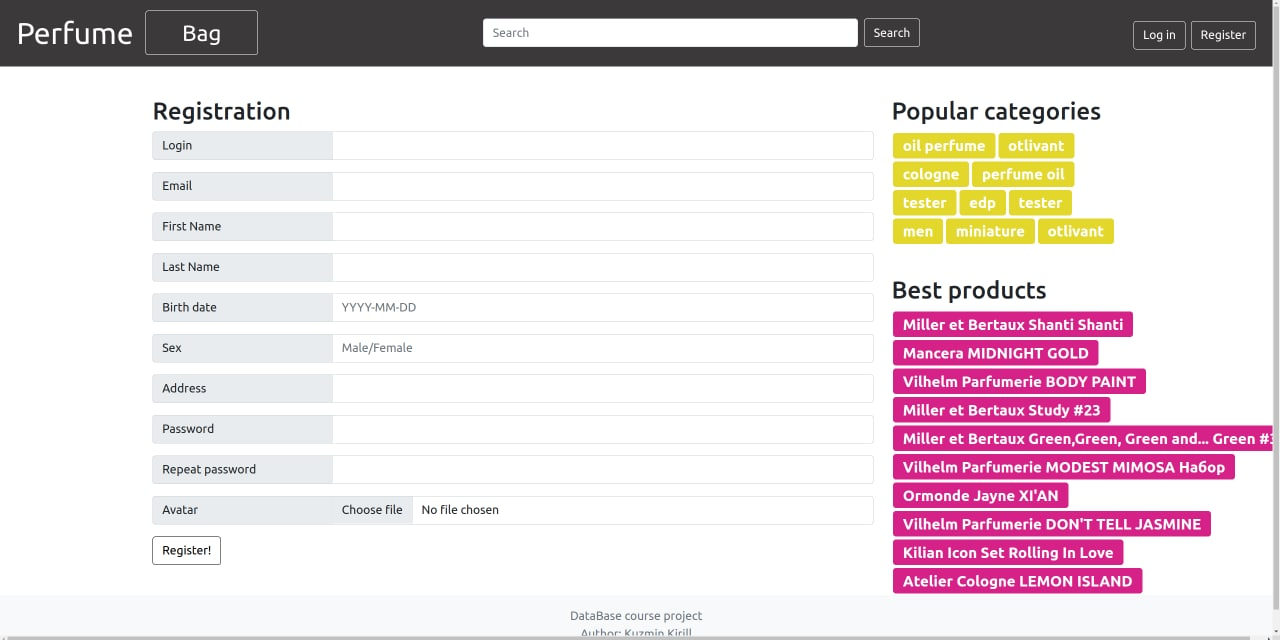
\includegraphics[scale=0.45]{assets/site_reg.jpg}
	\end{center}
	\caption{Страница регистрации}
	\label{site_reg}
\end{figure}

\subsection{Вход в систему}

На рисунке \ref{site_login} представлена страница входа в систему. Для авторизации необходимо ввести login и password пользователя, зарегистрированного в системе и нажать на кнопку "Login". При необходимости с этой страницы можно попасть на страницу регистрации, нажав кнопку "Create new account".

\captionsetup{singlelinecheck = false, justification=centering}
\begin{figure}[h!]
	\begin{center}
		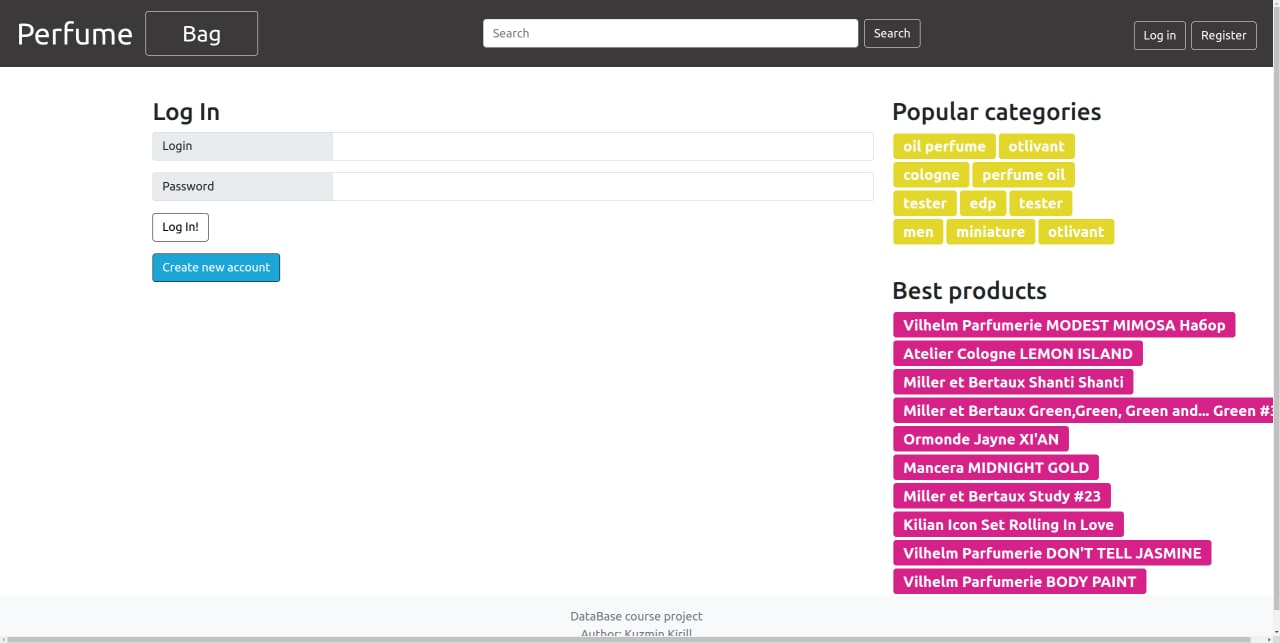
\includegraphics[scale=0.45]{assets/site_login.jpg}
	\end{center}
	\caption{Страница входа в систему}
	\label{site_login}
\end{figure}

\subsection{Изменение данных пользователя}

На рисунке \ref{site_settings} представлена страница, позволяющая изменять данные пользователя. Для этого пользователь должен изменить соответсвующие поля. Поле "avatar" не обязательно для заполнения. После изменения информации следует нажать на кнопку "save" чтобы изменения вступили в силу.

\captionsetup{singlelinecheck = false, justification=centering}
\begin{figure}[h!]
	\begin{center}
		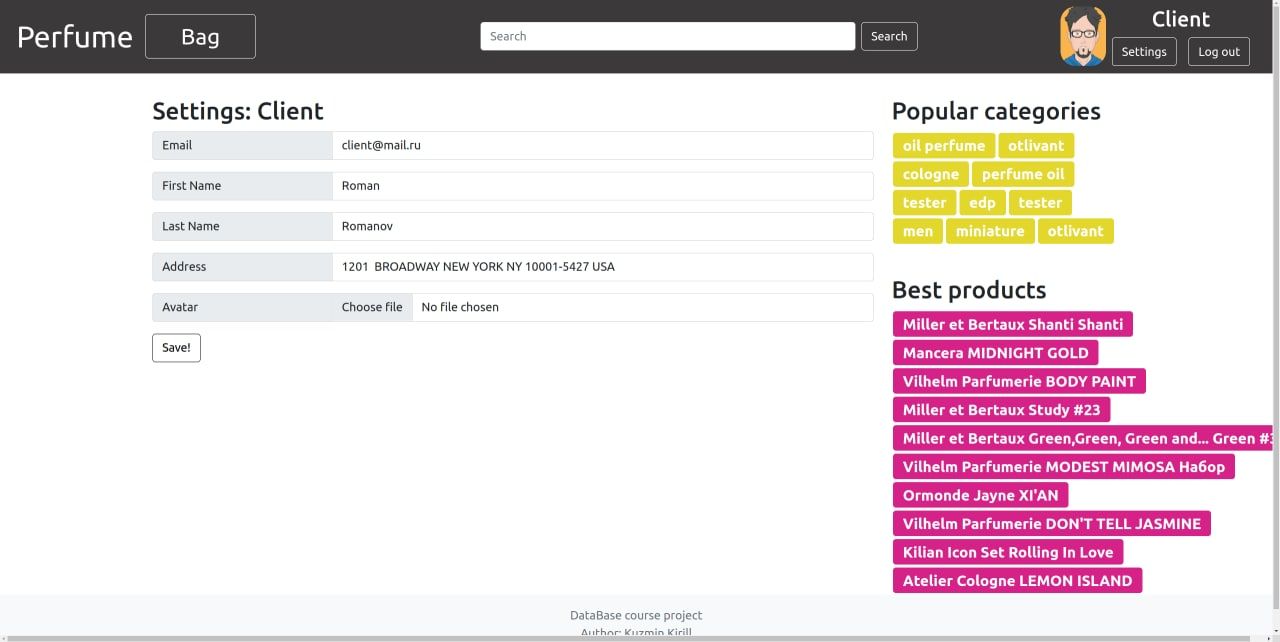
\includegraphics[scale=0.45]{assets/site_settings.jpg}
	\end{center}
	\caption{Страница изменения данных пользователя}
	\label{site_settings}
\end{figure}

\subsection{Поиск товаров}

На рисунке \ref{site_search} представлена страница с результатами поиска по строке "musk". Для выполнения поиска следует ввести поисковый запрос и нажать кнопку "Search". Поиск осуществляется по вхождению поискового запроса в название товара. Поиск не чувствителен к регистру.

\captionsetup{singlelinecheck = false, justification=centering}
\begin{figure}[h!]
	\begin{center}
		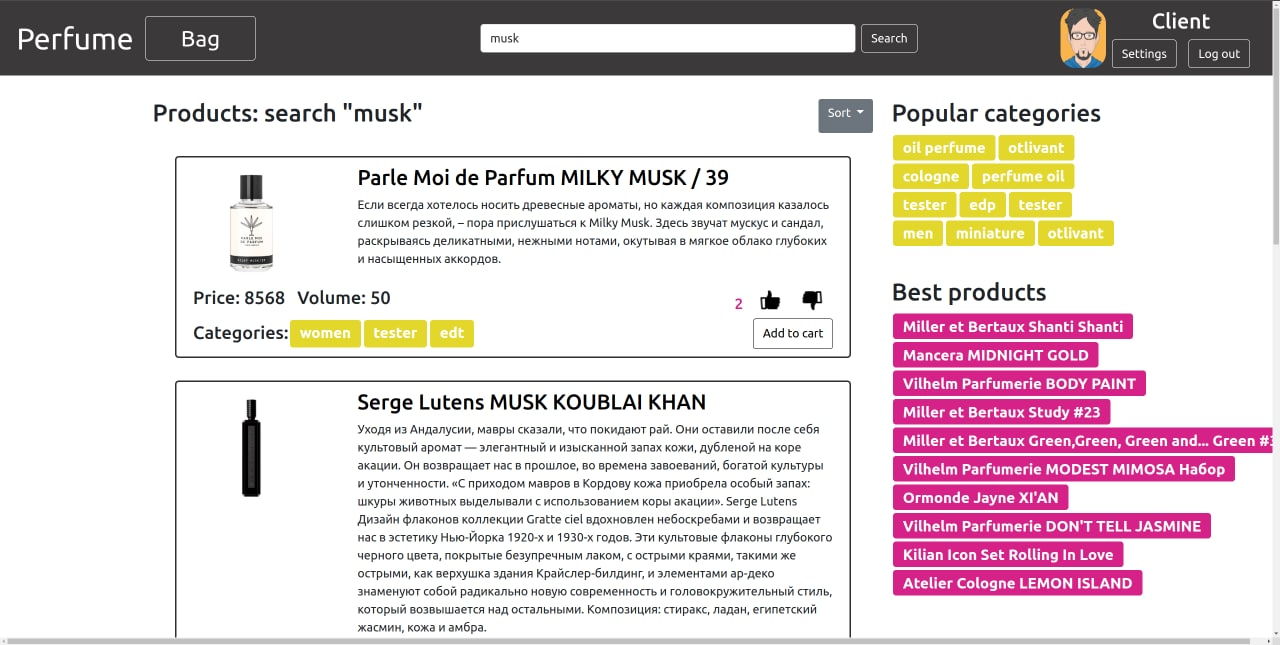
\includegraphics[scale=0.45]{assets/site_search.jpg}
	\end{center}
	\caption{Страница поиска товаров}
	\label{site_search}
\end{figure}

\subsection{Страница товара}

На рисунке \ref{site_product} представлена страница товара, на которой показано описание товара, цена, объем флакона, а также категории, к которым относится данный товар. Здесь можно поставить оценку товару в формате "нравится - не нравится". Чтобы добавить товар в корзину следует нажать кнопку "Add to cart". На странице товара представлены отзывы других пользователей на данный товар и оценки на отзывы, поставить которую можно так же, как и на товар. 

\captionsetup{singlelinecheck = false, justification=centering}
\begin{figure}[h!]
	\begin{center}
		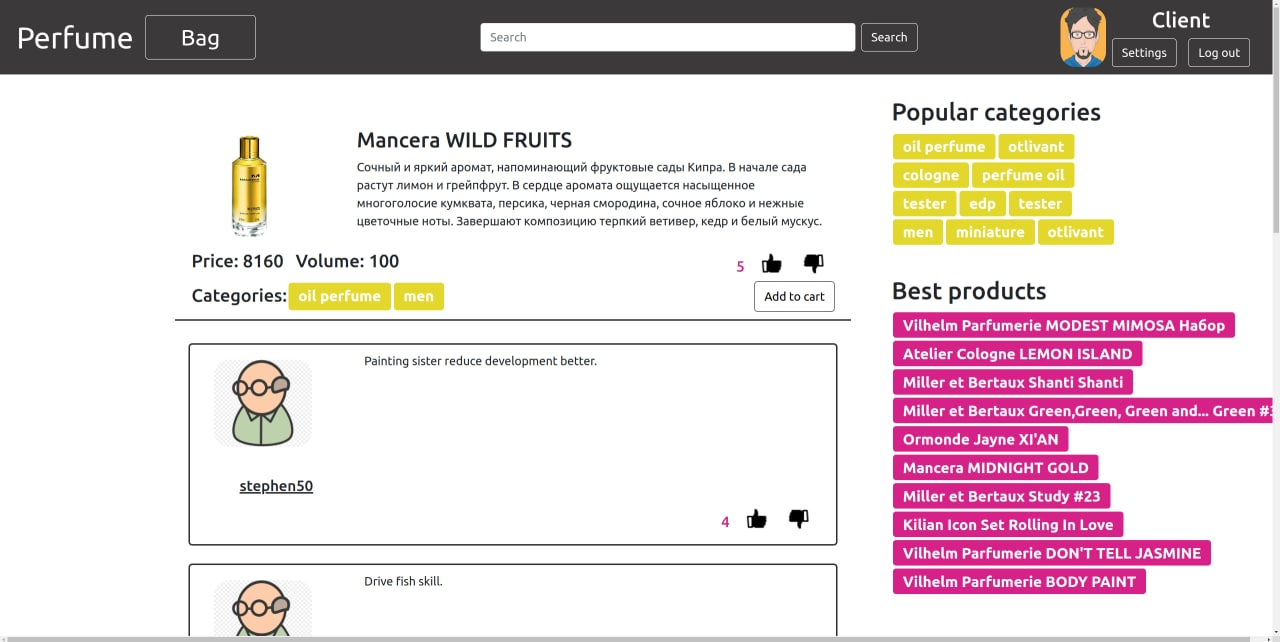
\includegraphics[scale=0.45]{assets/site_product.jpg}
	\end{center}
	\caption{Страница продукта}
	\label{site_product}
\end{figure}

\subsection{Создание отзыва}

На рисунке \ref{site_create_review} представлена страница создания отзыва. Для того, чтобы оставить отзыв пользователь должен войти в систему, зайти на страницу товара, заполнить форму Отзыва и нажать на кнопку "Review".

\captionsetup{singlelinecheck = false, justification=centering}
\begin{figure}[h!]
	\begin{center}
		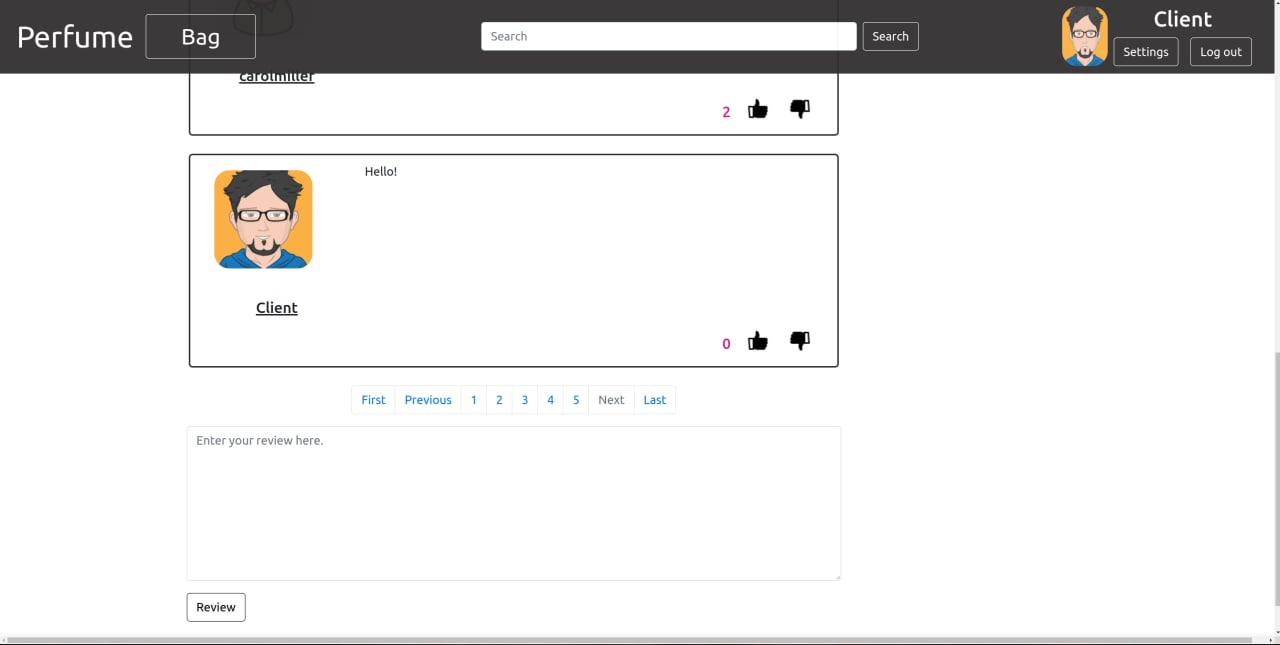
\includegraphics[scale=0.45]{assets/site_create_review.jpg}
	\end{center}
	\caption{Страница создания отзыва}
	\label{site_create_review}
\end{figure}

\subsection{Корзина товаров}

На рисунке \ref{site_bag} представлена страница с корзиной товаров, добавленных пользователем. Для изменения количества товара в корзине следует воспользоваться кнопками - и +, расположенными напротив наименования товара. Когда количество товара в корзине станет равным нулю, товар будет удален из корзины. На данной странице также показывается итоговая стоимость заказа. Чтобы просмотреть информацию о товаре из корзины следует нажать на название товара. Для просмотра истории заказов нужно нажать кнопку "Order history".

\captionsetup{singlelinecheck = false, justification=centering}
\begin{figure}[h!]
	\begin{center}
		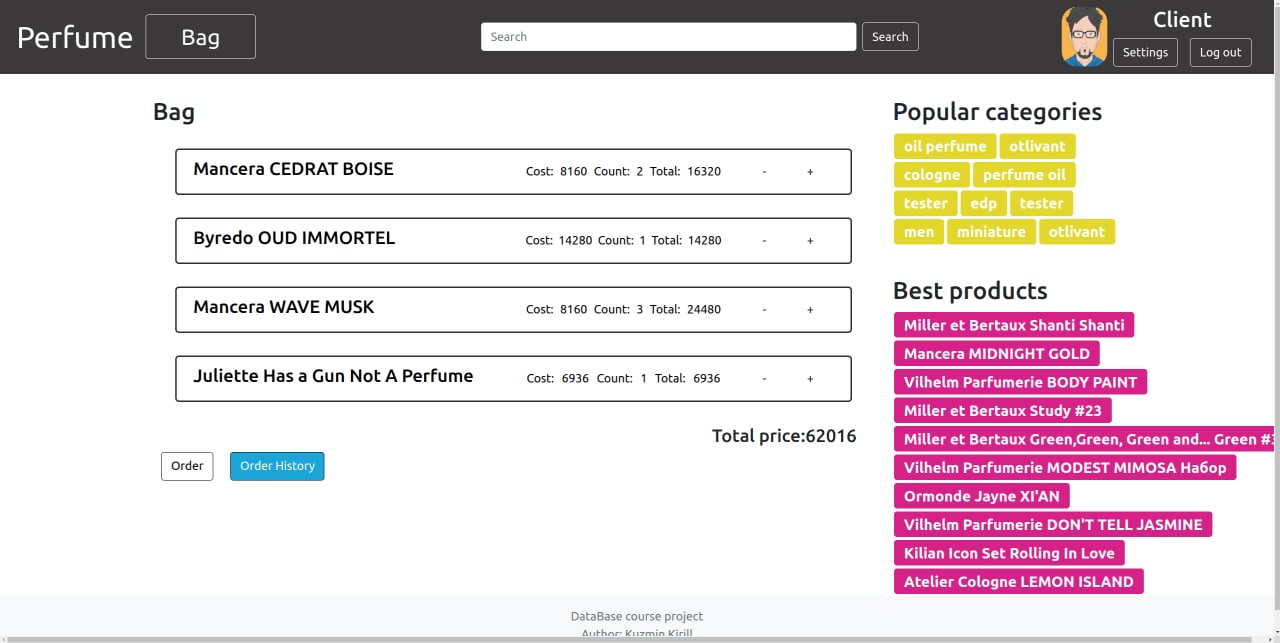
\includegraphics[scale=0.45]{assets/site_bag.jpg}
	\end{center}
	\caption{Корзина товаров}
	\label{site_bag}
\end{figure}

\subsection{История заказов пользователя}

На рисунке \ref{site_orders} представлена страница истории заказов пользователя. Для отображения подробной информации о заказе следует нажать на нужный заказ, пользователь будет перенаправлен на страницу заказа.

\captionsetup{singlelinecheck = false, justification=centering}
\begin{figure}[h!]
	\begin{center}
		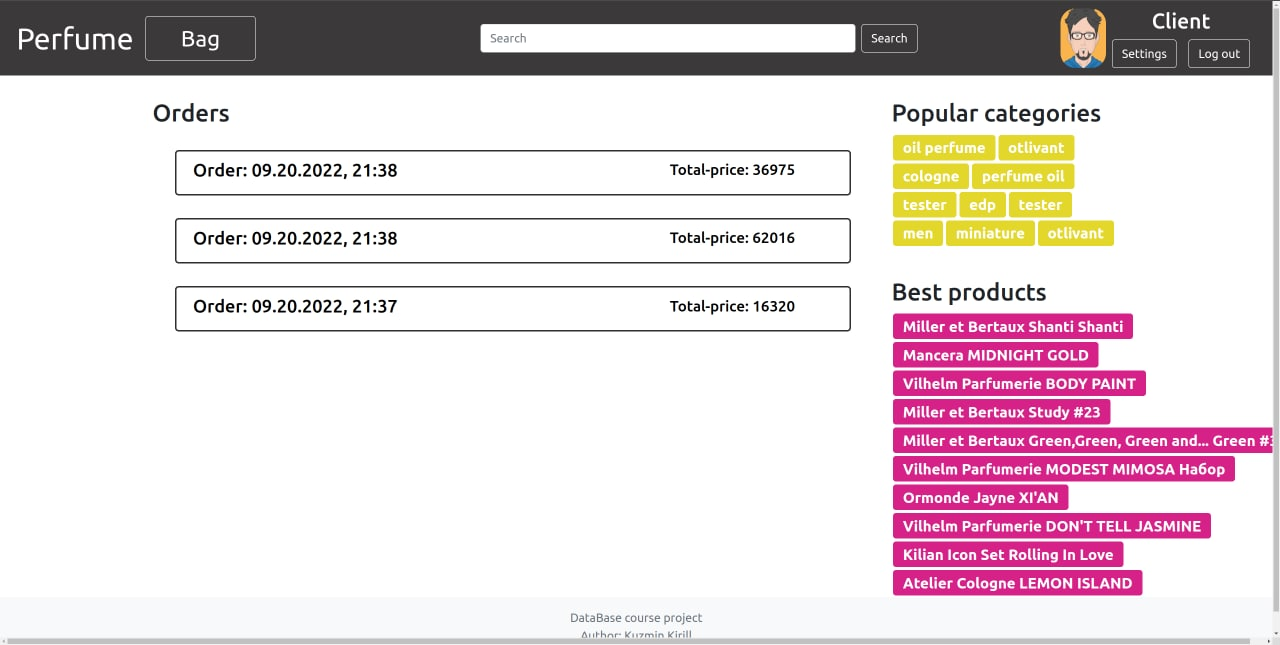
\includegraphics[scale=0.45]{assets/site_orders.jpg}
	\end{center}
	\caption{Страница истории заказов}
	\label{site_orders}
\end{figure}

\subsection{Страница управления товаром}

На рисунке \ref{site_admin_product} представлена страница управления товаром с аккаунта администратора. Доступ к данному функционалу имеется у пользователей с ролью manager и administrator. Данная страница позволяет изменять характеристики товара, создавать и удалять товары.

\captionsetup{singlelinecheck = false, justification=centering}
\begin{figure}[h!]
	\begin{center}
		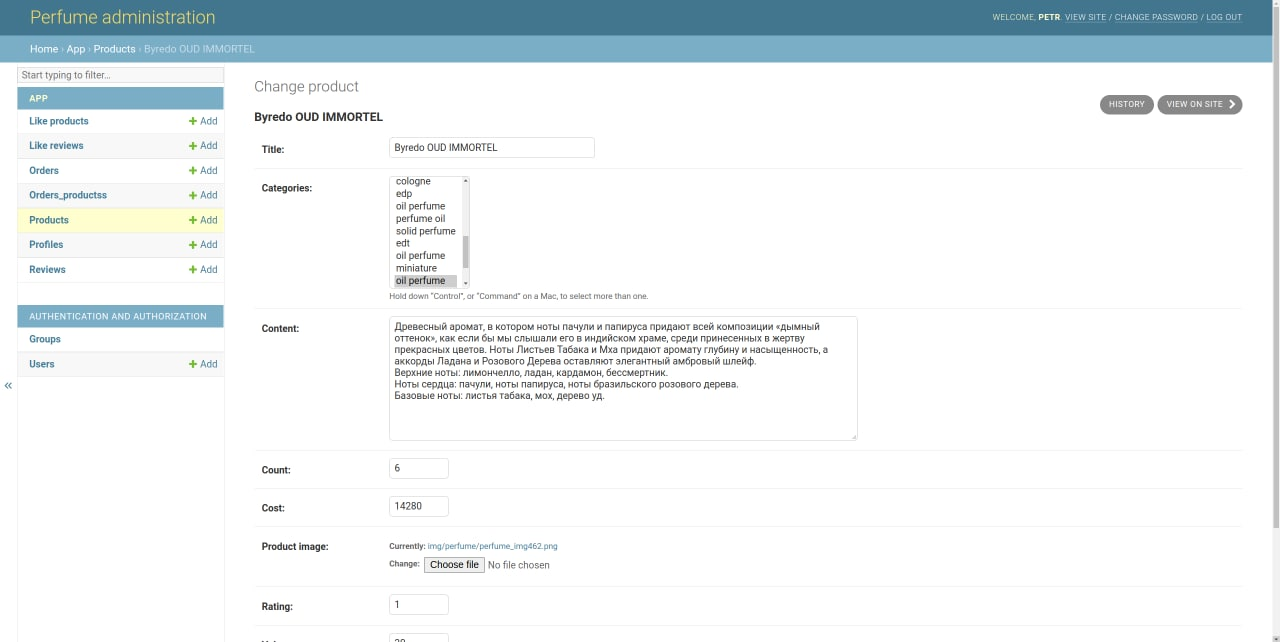
\includegraphics[scale=0.45]{assets/site_admin_product.jpg}
	\end{center}
	\caption{Страница управления товаром}
	\label{site_admin_product}
\end{figure}

\subsection{Страница управления пользователями}

На рисунке \ref{site_admin_users} представлена страница управления пользователями. Пользователи с ролью administrator могут вносить изменения в поля пользователей, удалять и создавать новых пользователей. Manager может просматривать информацию пользователей.

\captionsetup{singlelinecheck = false, justification=centering}
\begin{figure}[h!]
	\begin{center}
		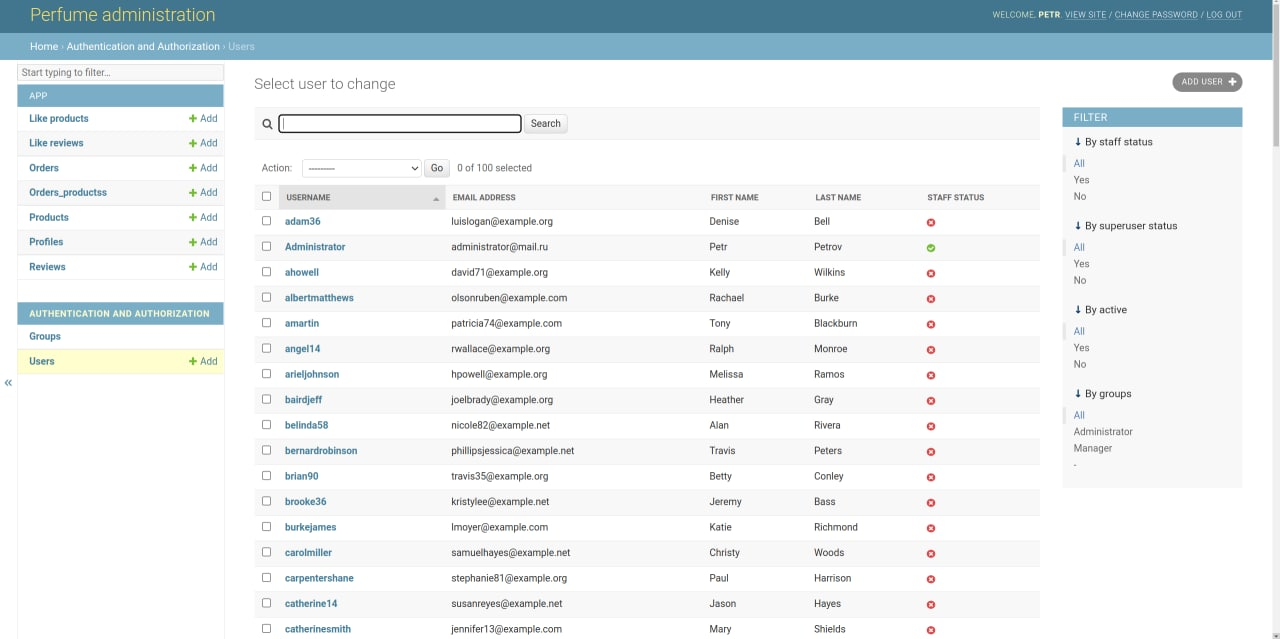
\includegraphics[scale=0.45]{assets/site_admin_users.jpg}
	\end{center}
	\caption{Страница управления пользователями}
	\label{site_admin_users}
\end{figure}